\documentclass{homework}
\usepackage{booktabs}
\usepackage{subfig}
% \captionsetup[subfigure]{labelformat=empty}


\usepackage{tikz}
\usepackage{pgf}
\usetikzlibrary{arrows,arrows.meta,matrix,shapes.geometric,automata}
\usepackage{xcolor}
\definecolor{mgreen}{HTML}{39825a}

\usepackage{amssymb}% http://ctan.org/pkg/amssymb
\usepackage{pifont}% http://ctan.org/pkg/pifont
\newcommand{\cmark}{\ding{51}}%
\newcommand{\xmark}{\ding{55}}%

\usepackage{fancyvrb,newverbs,xcolor}

% \usepackage[T1]{fontenc}
% \usepackage{mathabx,graphicx}
\def\Circlearrowleft{\ensuremath{%
  \rotatebox[origin=c]{180}{$\circlearrowleft$}}}
\def\Circlearrowright{\ensuremath{%
  \rotatebox[origin=c]{180}{$\circlearrowright$}}}
\def\CircleArrowleft{\ensuremath{%
  \reflectbox{\rotatebox[origin=c]{180}{$\circlearrowleft$}}}}
\def\CircleArrowright{\ensuremath{%
  \reflectbox{\rotatebox[origin=c]{180}{$\circlearrowright$}}}}
  
\def\clockwise{\circlearrowright}
\def\counterclockwise{\circlearrowleft}

\definecolor{cverbbg}{gray}{0.93}

\newenvironment{cverbatim}
 {\SaveVerbatim{cverb}}
 {\endSaveVerbatim
  \flushleft\fboxrule=0pt\fboxsep=.5em
  \colorbox{cverbbg}{\BUseVerbatim{cverb}}
  \endflushleft
}
\newenvironment{lcverbatim}
 {\SaveVerbatim{cverb}}
 {\endSaveVerbatim
  \flushleft\fboxrule=0pt\fboxsep=.5em
  \colorbox{cverbbg}{%
    \makebox[\dimexpr\linewidth-2\fboxsep][l]{\BUseVerbatim{cverb}}
  }
  \endflushleft
}

\newcommand{\ctexttt}[1]{\colorbox{cverbbg}{\texttt{#1}}}
\newverbcommand{\cverb}
  {\setbox\verbbox\hbox\bgroup}
  {\egroup\colorbox{cverbbg}{\box\verbbox}}

\title{CIS 571 - Assignment 3}
\author{Ali Hassani}

\begin{document}

\maketitle

\renewcommand{\theenumi}{\alph{enumi}}
\renewcommand{\theenumii}{\roman{enumii}}

\exercise[1]

\subsection{Part 1 - Cycle}
\begin{figure}[h!]
    \centering
    \begin{minipage}[b]{0.49\textwidth}
        \centering
        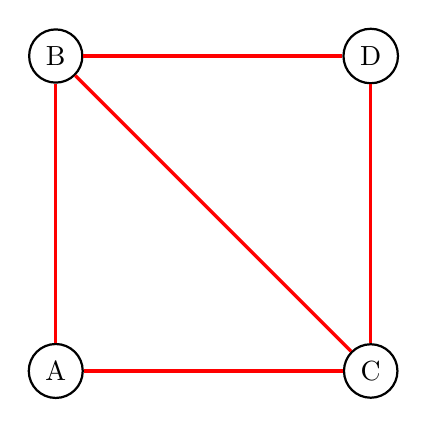
\begin{tikzpicture}
\begin{scope}[every node/.style={circle,thick,draw}]
    \node (A) at (0,0) {A};
    \node (B) at (0,4) {B};
    \node (C) at (4,0) {C};
    \node (D) at (4,4) {D};
\end{scope}

\begin{scope}[>={Stealth[black]},
              every node/.style={circle},
              every edge/.style={draw=red,very thick}]
    \path [-] (A) edge node {} (C);
    \path [-] (B) edge node {} (C);
    \path [-] (D) edge node {} (C);
    \path [-] (B) edge node {} (A);
    \path [-] (B) edge node {} (D);
\end{scope}
\end{tikzpicture}
    \end{minipage}
    % \hfill
    \begin{minipage}[b]{0.49\textwidth}
        \begin{tabular}{c|c|c|c|c}
            \toprule
            $s$ & $a$ & $s^{\prime}$ & $T(s, a, s^{\prime})$ & $R(s, a, s^{\prime})$ \\
            \midrule
            A & Clockwise & B & 1.0 & 0.0 \\
            A & Counterclockwise & C & 1.0 & -2.0 \\
            B & Clockwise & A & 0.4 & -1.0 \\
            B & Clockwise & C & 0.6 & 2.0 \\
            B & Counterclockwise & A & 0.6 & 2.0 \\
            B & Counterclockwise & C & 0.4 & -1.0 \\
            C & Clockwise & A & 0.6 & 2.0 \\
            C & Clockwise & B & 0.4 & 2.0 \\
            C & Counterclockwise & A & 0.4 & 2.0 \\
            C & Counterclockwise & B & 0.6 & 0.0 \\
            \bottomrule
        \end{tabular}
    \end{minipage}
    % \caption{MDP Transition diagram}
    \label{fig:q1}
\end{figure}
% \begin{figure}[h!]
%     \centering
%     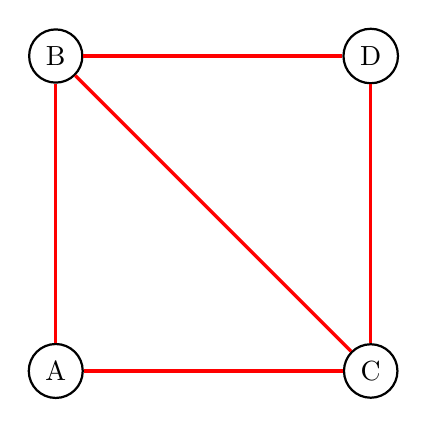
\begin{tikzpicture}
\begin{scope}[every node/.style={circle,thick,draw}]
    \node (A) at (0,0) {A};
    \node (B) at (0,4) {B};
    \node (C) at (4,0) {C};
    \node (D) at (4,4) {D};
\end{scope}

\begin{scope}[>={Stealth[black]},
              every node/.style={circle},
              every edge/.style={draw=red,very thick}]
    \path [-] (A) edge node {} (C);
    \path [-] (B) edge node {} (C);
    \path [-] (D) edge node {} (C);
    \path [-] (B) edge node {} (A);
    \path [-] (B) edge node {} (D);
\end{scope}
\end{tikzpicture}
%     \caption{MDP Transition diagram}
%     \label{fig:q11}
% \end{figure}

% \begin{table}[h!]
%     \centering
%     \begin{tabular}{c|c|c|c|c}
%         \toprule
%         $s$ & $a$ & $s^{\prime}$ & $T(s, a, s^{\prime})$ & $R(s, a, s^{\prime})$ \\
%         \midrule
%         A & Clockwise & B & 1.0 & 0.0 \\
%         A & Counterclockwise & C & 1.0 & -2.0 \\
%         B & Clockwise & A & 0.4 & -1.0 \\
%         B & Clockwise & C & 0.6 & 2.0 \\
%         B & Counterclockwise & A & 0.6 & 2.0 \\
%         B & Counterclockwise & C & 0.4 & -1.0 \\
%         C & Clockwise & A & 0.6 & 2.0 \\
%         C & Clockwise & B & 0.4 & 2.0 \\
%         C & Counterclockwise & A & 0.4 & 2.0 \\
%         C & Counterclockwise & B & 0.6 & 0.0 \\
%         \bottomrule
%     \end{tabular}
%     \caption{Transition \& reward functions}
%     \label{tab:q11trf}
% \end{table}
$\gamma = 0.5$.
\clearpage
\textbf{\large P1.1. Suppose after iteration $k$, we obtain the values below. Provide values at $k+1$.}

\begin{table}[h!]
    \centering
    \begin{tabular}{c|c|c}
        \toprule
        $V_k(A)$ & $V_k(B)$ & $V_k(C)$ \\
        \midrule
        0.400 & 1.400 & 2.160 \\
        \bottomrule
    \end{tabular}
    \label{tab:q1avk}
\end{table}
For $s \in \{ A, B, C \}$, $V_{k+1}(s) = \max\limits_{a} Q_{k+1}(s, a)$, and $Q_{k+1}(s, a) = \sum\limits_{s^{\prime}}{ T(s, a, s^{\prime})[ R(s, a, s^{\prime}) + \gamma V_{k}(s^{\prime}) ] }$. Therefore:

\begin{table}[h!]
    \centering
    \begin{tabular}{lccc}
        \toprule
         & $A$ & $B$ & $C$ \\
        \midrule
        $\clockwise$ & 0.70 & 1.53 & 2.40 \\
        $\counterclockwise$ & -0.92  & 1.35 & 1.30 \\
        \bottomrule
    \end{tabular}
    \caption{$Q_{k+1}$}
    \label{tab:q11aqkp1}
\end{table}
Therefore:
\begin{table}[h!]
    \centering
    \begin{tabular}{c|c|c}
        \toprule
        $V_{k+1}(A)$ & $V_{k+1}(B)$ & $V_{k+1}(C)$ \\
        \midrule
        0.70 & 1.53 & 2.40 \\
        \bottomrule
    \end{tabular}
    \label{tab:q11avkp1}
\end{table}

\textbf{\large P1.2. Suppose that we ran value iteration to completion and found the following value function, $V^{*}$. What are the optimal actions from states $A$, $B$, and $C$, respectively?}

\begin{table}[h!]
    \centering
    \begin{tabular}{c|c|c}
        \toprule
        $V^{\star}(A)$ & $V^{\star}(B)$ & $V^{\star}(C)$ \\
        \midrule
        0.881 & 1.761 & 2.616 \\
        \bottomrule
    \end{tabular}
    \label{tab:q1str}
\end{table}
For $s \in \{ A, B, C \}$, $V^{\star}(s) = \max\limits_{a} Q^{\star}(s, a)$, and $Q^{\star}(s, a) = \sum\limits_{s^{\prime}}{ T(s, a, s^{\prime})[ R(s, a, s^{\prime}) + \gamma V^{\star}(s^{\prime}) ] }$ (convergence of value iteration). Therefore:

\begin{table}[h!]
    \centering
    \begin{tabular}{lccc}
        \toprule
         & $A$ & $B$ & $C$ \\
        \midrule
        $\clockwise$ & \textbf{0.8805} & \textbf{1.7610} & \textbf{2.6165} \\
        $\counterclockwise$ & -0.6920  & 1.5875 & 1.5045 \\
        \bottomrule
    \end{tabular}
    \caption{$Q^{\star}$}
    \label{tab:q12aqkp1}
\end{table}
Therefore, the optimal action at every state is moving clockwise.

\clearpage
\subsection{Part 2 - Convergence}
For all transitions from any state to another, reward is $1$. From $F$, there is no transition to another state, just to itself, the reward for which is $0$.
\begin{figure}[h!]
    \centering
    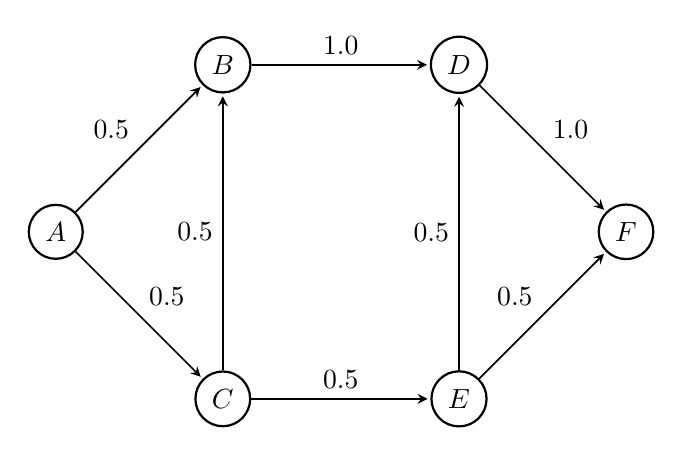
\begin{tikzpicture}[
        > = stealth, % arrow head style
        shorten > = 1pt, % don't touch arrow head to node
        auto,
        node distance = 3cm, % distance between nodes
        semithick % line style
    ]

    \tikzstyle{every state}=[
        draw = black,
        thick,
        fill = white,
        minimum size = 4mm
    ]

    \node[state] (A) {$A$};
    \node[state] (B) [above right of=A] {$B$};
    \node[state] (C) [below right of=A] {$C$};
    \node[state] (D) [right of=B] {$D$};
    \node[state] (E) [right of=C] {$E$};
    \node[state] (F) [below right of=D] {$F$};

    \path[->] (A) edge node {0.5} (B);
    \path[->] (A) edge node {0.5} (C);
    \path[->] (B) edge node {1.0} (D);
    \path[->] (C) edge node {0.5} (B);
    \path[->] (C) edge node {0.5} (E);
    \path[->] (D) edge node {1.0} (F);
    \path[->] (E) edge node {0.5} (D);
    \path[->] (E) edge node {0.5} (F);
\end{tikzpicture}

    \caption{Transition diagram}
    \label{fig:q12}
\end{figure}

\textbf{\large P2.1. After how many iterations of value iteration will the value for state $E$ have become exactly equal to the true optimum? (Enter inf if the values will never become equal to the true optimal but only converge to the true optimal.)}

After 2 iterations. To explicitly check: after the first iteration, $V_{1}(E) = 1.0$, and after the second, $V_{2}(E) = 1.25$.

\textbf{\large P2.2. How many iterations of value iteration will it take for the values of all states to converge to the true optimal values? (Enter inf if the values will never become equal to the true optimal but only converge to the true optimal.)}

After 4 iterations. To explicitly check:

\begin{table}[h!]
    \centering
    \begin{tabular}{c|c|c|c|c|c}
        \toprule
        $V^{\star}(A)$ & $V^{\star}(B)$ & $V^{\star}(C)$ & $V^{\star}(D)$ & $V^{\star}(E)$ & $V^{\star}(F)$ \\
        \midrule
        1.796875 & 1.500000 & 1.687500 & 1.000000 & 1.250000 & 0.000000 \\
        \bottomrule
    \end{tabular}
    \label{tab:q12vstr}
\end{table}

\clearpage
\exercise[2]
\begin{figure}[h!]
    \centering
    \begin{minipage}[b]{0.49\textwidth}
        \centering
        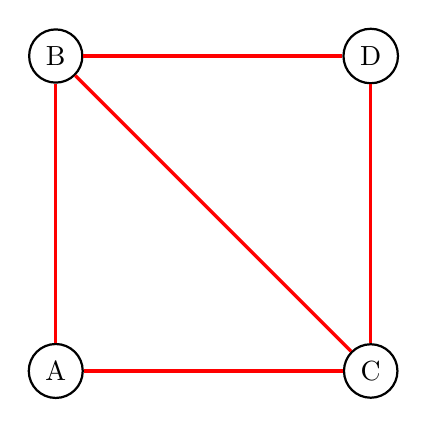
\begin{tikzpicture}
\begin{scope}[every node/.style={circle,thick,draw}]
    \node (A) at (0,0) {A};
    \node (B) at (0,4) {B};
    \node (C) at (4,0) {C};
    \node (D) at (4,4) {D};
\end{scope}

\begin{scope}[>={Stealth[black]},
              every node/.style={circle},
              every edge/.style={draw=red,very thick}]
    \path [-] (A) edge node {} (C);
    \path [-] (B) edge node {} (C);
    \path [-] (D) edge node {} (C);
    \path [-] (B) edge node {} (A);
    \path [-] (B) edge node {} (D);
\end{scope}
\end{tikzpicture}
    \end{minipage}
    % \hfill
    \begin{minipage}[b]{0.49\textwidth}
        \begin{tabular}{c|c|c|c|c}
            \toprule
            $s$ & $a$ & $s^{\prime}$ & $T(s, a, s^{\prime})$ & $R(s, a, s^{\prime})$ \\
            \midrule
            A & Clockwise & B & 1.0 & 0.0 \\
            A & Counterclockwise & C & 1.0 & -2.0 \\
            B & Clockwise & A & 0.4 & -1.0 \\
            B & Clockwise & C & 0.6 & 2.0 \\
            B & Counterclockwise & A & 0.6 & 2.0 \\
            B & Counterclockwise & C & 0.4 & -1.0 \\
            C & Clockwise & A & 0.6 & 2.0 \\
            C & Clockwise & B & 0.4 & 2.0 \\
            C & Counterclockwise & A & 0.4 & 2.0 \\
            C & Counterclockwise & B & 0.6 & 0.0 \\
            \bottomrule
        \end{tabular}
    \end{minipage}
    % \caption{MDP Transition diagram}
    \label{fig:q2}
\end{figure}

\begin{table}[h!]
    \centering
    \caption{Transition \& reward functions}
    \label{tab:q2}
\end{table}
$\gamma = 0.5$.

\subsection{Suppose we are doing policy evaluation, by following the policy given by the left-hand side table below. Our current estimates (at the end of some iteration of policy evaluation) of the value of states when following the current policy is given in the right-hand side table.}

\begin{table}[h!]
    \centering
    \begin{tabular}{c|c|c}
        \toprule
        $A$ & $B$ & $C$ \\
        \midrule
        Counterclockwise & Counterclockwise & Counterclockwise \\
        \bottomrule
    \end{tabular}
    \hfill
    \begin{tabular}{c|c|c}
        \toprule
        $V^{\pi}_{k+1}(A)$ & $V^{\pi}_{k+1}(B)$ & $V^{\pi}_{k+1}(C)$ \\
        \midrule
        $0.000$ & $-0.840$ & $-1.080$ \\
        \bottomrule
    \end{tabular}
\end{table}

\textbf{\large Provide the value of $V^{\pi}_{k+1}(A)$, $V^{\pi}_{k+1}(B)$, and $V^{\pi}_{k+1}(C)$.}
\begin{table}[h!]
    \centering
    \begin{tabular}{c|c|c}
        \toprule
        $V^{\pi}_{k+1}(A)$ & $V^{\pi}_{k+1}(B)$ & $V^{\pi}_{k+1}(C)$ \\
        \midrule
        $-2.540$ & $0.584$ & $0.548$ \\
        \bottomrule
    \end{tabular}
\end{table}

\clearpage
\subsection{Suppose that policy evaluation converges to the following value function.}

\begin{table}[h!]
    \centering
    \begin{tabular}{c|c|c}
        \toprule
        $V_{\infty}^{\pi}(A)$ & $V_{\infty}^{\pi}(B)$ & $V_{\infty}^{\pi}(C)$ \\
        \midrule
        $-0.203$ & $-1.114$ & $-1.266$ \\
        \bottomrule
    \end{tabular}
\end{table}

\textbf{\large Provide the values of $Q_{\infty}^{\pi}(A, \clockwise)$ and $Q_{\infty}^{\pi}(A, \counterclockwise)$. What is the updated action for $A$?}

The $V_{\infty}$s above lead to the following $Q_{\infty}$s:

\begin{table}[h!]
    \centering
    \begin{tabular}{cccc}
        \toprule
        & $Q_{\infty}^{\pi}(A)$ & $Q_{\infty}^{\pi}(B)$ & $Q_{\infty}^{\pi}(C)$ \\
        \midrule
        $\clockwise$ & $-0.56$ & $0.38$ & $1.72$ \\
        $\counterclockwise$ & $-2.63$ & $0.49$ & $0.42$ \\
        \bottomrule
    \end{tabular}
\end{table}

(Note that this contradicts the assumption that the values converged, because at least one policy from this $Q$ should have been approximately equal to the values provided. In other words, )

$Q_{\infty}^{\pi}(A, \clockwise) = -0.56$

$Q_{\infty}^{\pi}(A, \counterclockwise) = -2.63$

Therefore, the updated action for $A$ would be \textbf{Clockwise} ($\clockwise$).

\clearpage
\exercise[3]
\begin{figure}[h!]
    \centering
    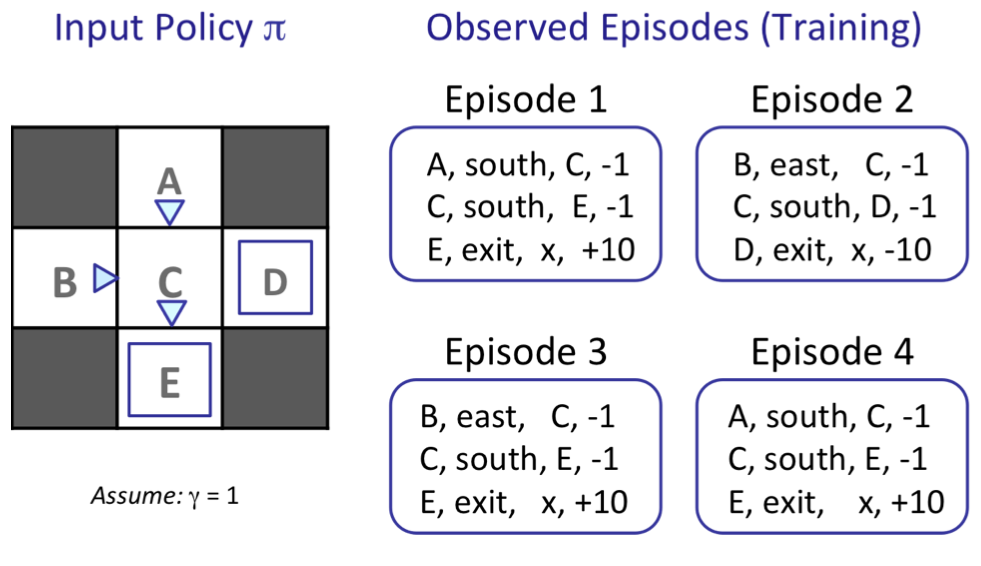
\includegraphics[width=0.8\textwidth]{figures/q3.png}
    \caption{Q3}
    \label{fig:q3}
\end{figure}
\textbf{\large What model would be learned from the above observed episodes (transition/reward functions)?}

% \begin{table}[h!]
%     \centering
%     \begin{tabular}{c|c|c|c|c}
%         \toprule
%         $s$ & $a$ & $s^{\prime}$ & $R(s, a, s^{\prime})$ \\
%         \midrule
%         A & south & C & -1 \\
%         A & south & C & -1 \\
%         B & east & C & -1 \\
%         B & east & C & -1 \\
%         C & south & D & -1 \\
%         C & south & E & -1 \\
%         C & south & E & -1 \\
%         C & south & E & -1 \\
%         D & exit & x & -10 \\
%         E & exit & x & +10 \\
%         E & exit & x & +10 \\
%         E & exit & x & +10 \\
%         \bottomrule
%     \end{tabular}
%     \caption{Sorted observations}
%     \label{tab:q3obs}
% \end{table}

\begin{table}[h!]
    \centering
    \begin{tabular}{c|c|c|c|c}
        \toprule
        $s$ & $a$ & $s^{\prime}$ & $T(s, a, s^{\prime})$ & $R(s, a, s^{\prime})$ \\
        \midrule
        A & south & C & 1.0 & -1 \\
        B & east & C & 1.0 & -1 \\
        C & south & D & 0.25 & -1 \\
        C & south & E & 0.75 & -1 \\
        D & exit & x & 1.0 & -10 \\
        E & exit & x & 1.0 & +10 \\
        \bottomrule
    \end{tabular}
    \caption{Learned transition \& reward functions}
    \label{tab:q3model}
\end{table}

\clearpage
\exercise[4]
\begin{figure}[h!]
    \centering
    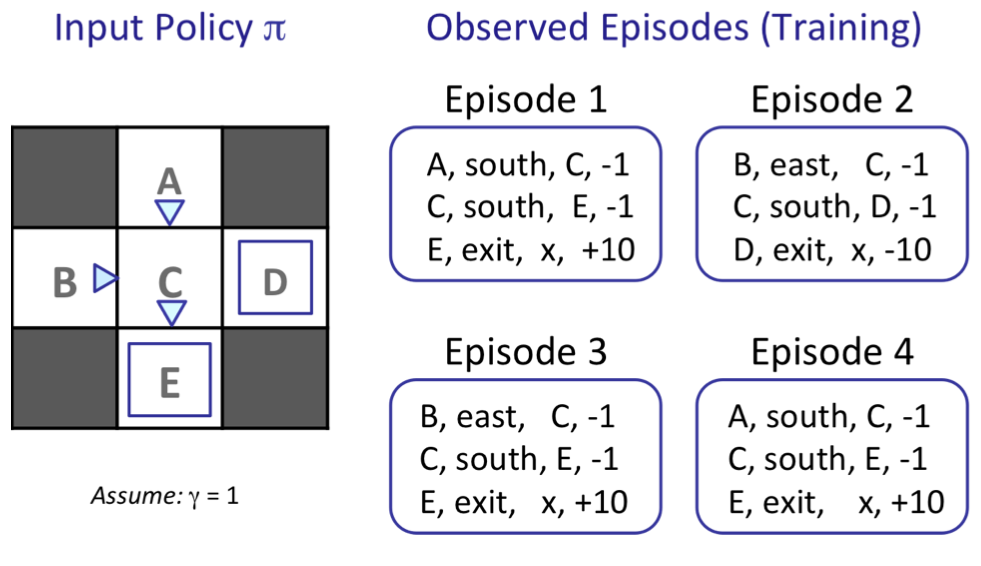
\includegraphics[width=0.8\textwidth]{figures/q3.png}
    \caption{Q4}
    \label{fig:q4}
\end{figure}
\textbf{\large What are the estimates for $V^{\pi}(A)$, $V^{\pi}(B)$, $V^{\pi}(C)$, $V^{\pi}(D)$, $V^{\pi}(E)$ as obtained by direct evaluation?}

\begin{table}[h!]
    \centering
    \begin{tabular}{c|c|c|c|c}
        \toprule
        $\hat{V}^{\pi}(A)$ & $\hat{V}^{\pi}(B)$ & $\hat{V}^{\pi}(C)$ & $\hat{V}^{\pi}(D)$ & $\hat{V}^{\pi}(E)$ \\
        \midrule
        8 & -2 & 4 & -10 & 10\\
        \bottomrule
    \end{tabular}
\end{table}

\clearpage
\exercise[5]
Consider the gridworld shown below. The left panel shows the name of each state $A$ through $E$. The middle panel shows the current estimate of the value function $V^{\pi}$ for each state. A transition is observed, that takes the agent from state $B$ through taking action east into state $C$, and the agent receives a reward of $-2$. Assuming $\gamma = 1$, $\alpha = 0.5$, what are the value estimates of $V^{\pi}(A)$, $V^{\pi}(B)$, $V^{\pi}(C)$, $V^{\pi}(D)$, and $V^{\pi}(E)$ after the TD learning update?
\begin{figure}[h!]
    \centering
    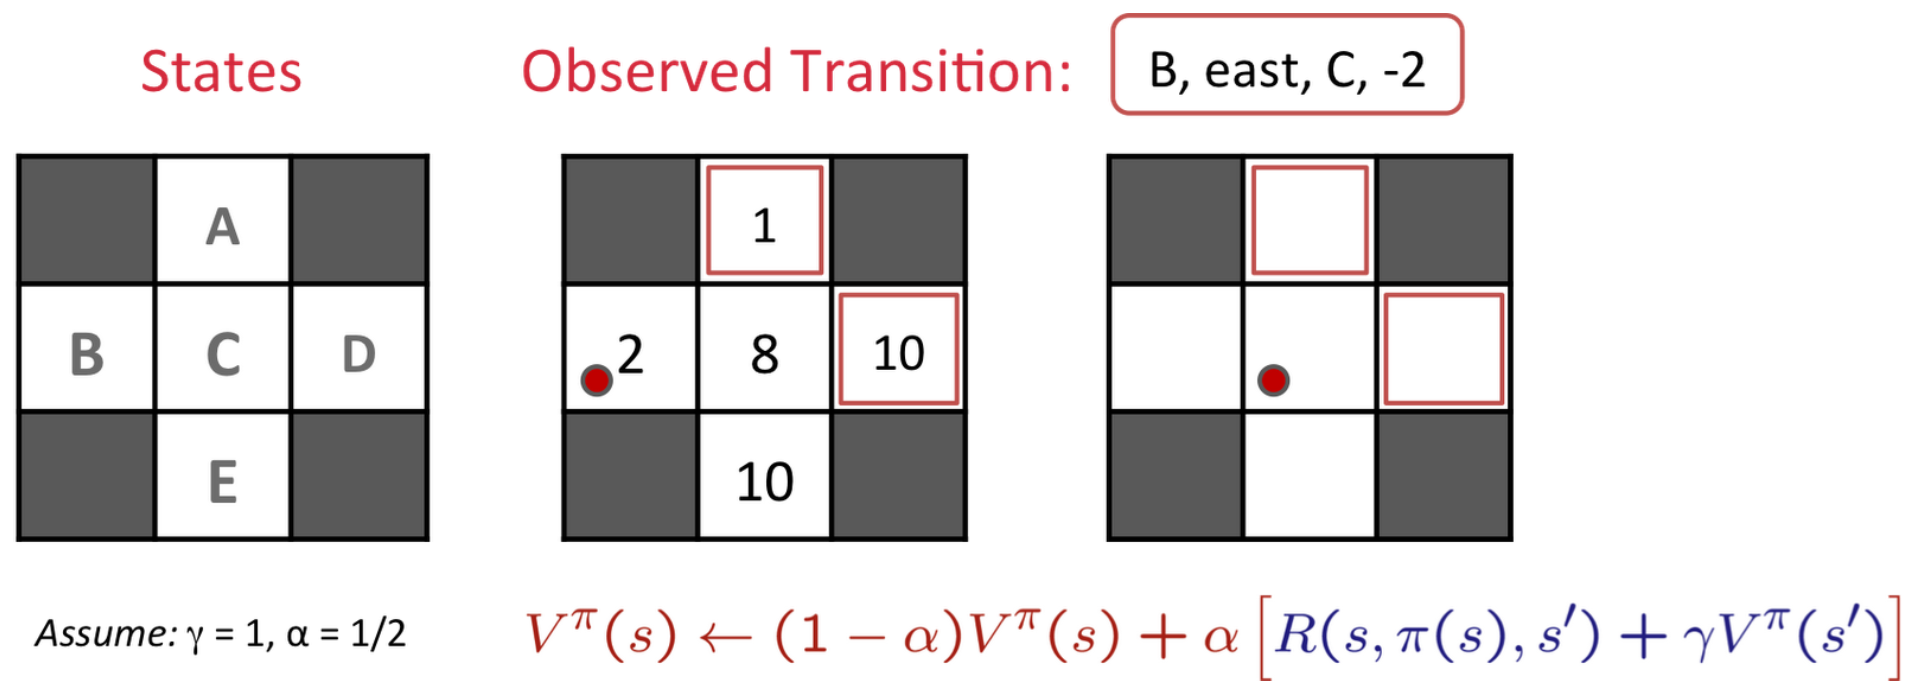
\includegraphics[width=0.8\textwidth]{figures/q5.png}
    \caption{Q5}
    \label{fig:q5}
\end{figure}
\begin{table}[h!]
    \centering
    \begin{tabular}{c|c|c|c|c}
        \toprule
        $V^{\pi}(A)$ & $V^{\pi}(B)$ & $V^{\pi}(C)$ & $V^{\pi}(D)$ & $V^{\pi}(E)$ \\
        \midrule
        1 & 2 & 8 & 10 & 10\\
        \bottomrule
    \end{tabular}
\end{table}

$V^{\pi}(B) = (1 - \alpha) V^{\pi}(B) + \alpha [ -2 + V^{\pi}(C) ] = 4$

Only $V^{\pi}(B)$ is updated from $2$ to $4$, the rest of the values stay the same.

\clearpage
\exercise[6]
Consider an MDP with 3 states: $A$, $B$ and $C$; and 2 actions Clockwise and Counterclockwise. We do not know the transition function or the reward function for the MDP, but instead, we are given with samples of what an agent actually experiences when it interacts with the environment (although, we do know that we do not remain in the same state after taking an action). In this problem, instead of first estimating the transition and reward functions, we will directly estimate the Q function using Q-learning. Assume, the discount factor, $\gamma$ is $0.75$ and the step size for Q-learning, $\alpha$ is $0.75$.
Our current Q function, Q(s, a), is shown in the left figure. The agent encounters the samples shown in the right figure:
\begin{table}[h!]
    \centering
    \begin{tabular}{cccc}
        \toprule
        & $A$ & $B$ & $C$ \\
        \midrule
        $\clockwise$ & 1.501 & -0.451 & 2.730 \\
        $\counterclockwise$ & 3.153 & -6.055 & 2.133 \\
        \bottomrule
    \end{tabular}
    \qquad
    \begin{tabular}{cccc}
        \toprule
        $s$ & $a$ & $s^{\prime}$ & $r$ \\
        \midrule
        $A$ & $\counterclockwise$ & C & 8.0 \\
        $C$ & $\counterclockwise$ & A & 0.0 \\
        \bottomrule
    \end{tabular}
\end{table}

\textbf{Provide the Q-values for all pairs of (state, action) after both samples have been accounted for.}

Assuming it is a batch-wise update (not sample-wise, because $Q(C, \counterclockwise)$ depends on the value of $Q(A, \counterclockwise)$ which is being updated):

\begin{equation*}
    Q(A, \counterclockwise) \Leftarrow (1 - \alpha) Q(A, \counterclockwise) + \alpha (sample)
\end{equation*}
\begin{align*}
    Q(A, \counterclockwise) &= (0.25 \times 3.153 ) + (0.75) \times ( 8.0 + (0.75 \times \max\limits_{a^{\prime}} Q(C, a^{\prime})) )\\
     &= (0.25 \times 3.153 ) + (0.75) \times ( 8.0 + (0.75 \times 2.730) )\\
     &= (0.78825) + (0.75) \times ( 8.0 + 2.0475 )\\
     &= (0.78825) + (0.75) \times ( 10.0475 )\\
     &= 0.78825 + 7.535625\\
     &= 8.323875\\
\end{align*}
\begin{align*}
    Q(C, \counterclockwise) &= (0.25 \times 2.133 ) + (0.75) \times ( 0.0 + (0.75 \times \max\limits_{a^{\prime}} Q(A, a^{\prime})) )\\
     &= (0.25 \times 2.133 ) + (0.75) \times ( (0.75 \times 3.153) )\\
     &= 0.53325 + 1.7735625\\
     &= 2.3068125\\
\end{align*}
Updated Q-values:
\begin{table}[h!]
    \centering
    \begin{tabular}{cccc}
        \toprule
        & $A$ & $B$ & $C$ \\
        \midrule
        $\clockwise$ & 1.501 & -0.451 & 2.730 \\
        $\counterclockwise$ & \textbf{\textcolor{blue}{8.323875}} & -6.055 & \textbf{\textcolor{blue}{2.3068125}} \\
        \bottomrule
    \end{tabular}
\end{table}

Assuming it is NOT a batch-wise update (it is sample-wise), $Q(C, \counterclockwise)$ would be computed as follows:
\begin{align*}
    Q(C, \counterclockwise) &= (0.25 \times 2.133 ) + (0.75) \times ( 0.0 + (0.75 \times \max\limits_{a^{\prime}} Q(A, a^{\prime})) )\\
     &= (0.25 \times 2.133 ) + (0.75) \times ( (0.75 \times 8.323875) )\\
     &= 0.53325 + 4.6821796875\\
     &= 5.21543\\
\end{align*}

Updated Q-values:
\begin{table}[h!]
    \centering
    \begin{tabular}{cccc}
        \toprule
        & $A$ & $B$ & $C$ \\
        \midrule
        $\clockwise$ & 1.501 & -0.451 & 2.730 \\
        $\counterclockwise$ & \textbf{\textcolor{blue}{8.323875}} & -6.055 & \textbf{\textcolor{blue}{5.21543}} \\
        \bottomrule
    \end{tabular}
\end{table}

\clearpage
\exercise[7]
Consider the following feature based representation of the Q-function: $Q(s, a) = w_1f_1(s, a) + w_2f_2(s, a)$ with:
\begin{itemize}
    \item $f_1(s, a) = \frac{1}{\text{Manhattan distance to nearest dot after having executed action }a\text{ in state }s)}$
    \item $f_2(s, a) =$ Manhattan distance to nearest ghost after having executed action $a$ in state $s$
\end{itemize}
Assuming $w_1 = 2$ and $w_2 = 8$,

\subsection{Assume that the red and blue ghosts are both sitting on top of a dot. Provide the following values. Based on them, which action would be chosen.}
\textbf{\large $ Q(s, west)$ and $Q(s, south)$.}

\begin{figure}[h!]
    \centering
    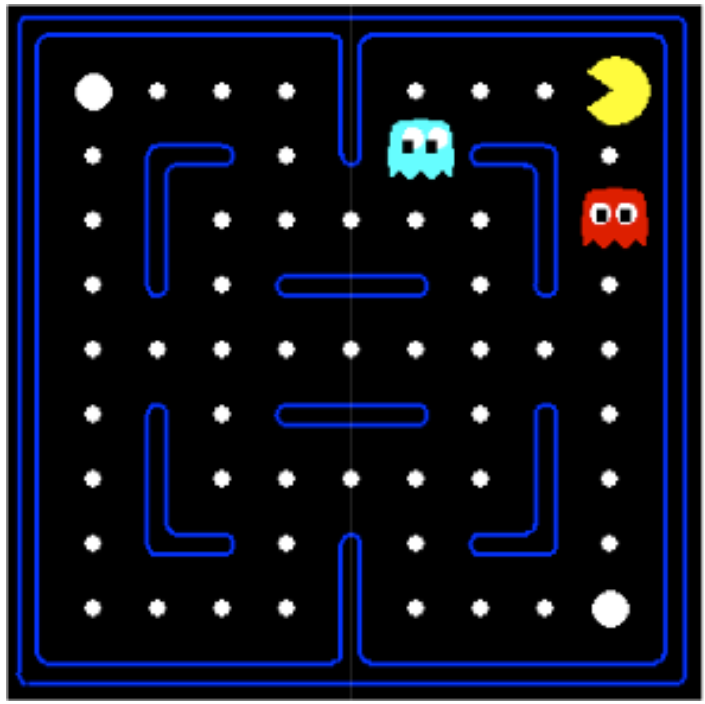
\includegraphics[width=0.35\textwidth]{figures/q71.png}
\end{figure}
Given that pacman is currently at state $s$:
\begin{align*}
    f_1(s, west) &= \frac{1}{1} = 1 \\
    f_2(s, west) &= 3 \\
    f_1(s, south) &= \frac{1}{2} = 0.5 \\
    f_2(s, south) &= 1 \\
\end{align*}
Therefore:
\begin{align*}
    Q(s, west) &= 1 \times 2 + 3 \times 8 = 26 \\
    Q(s, south) &= 0.5 \times 2 + 1 \times 8 = 9 \\
\end{align*}
Therefore, action $west$ will be chosen.

\clearpage
\subsection{Assume Pac-Man moves West. This results in the state shown below. Pac-Man receives reward 9 (10 for eating a dot and -1 living penalty).}
\textbf{\large Provide the values of $Q(s^{\prime}, west)$ and $Q(s^{\prime}, east)$. What is the sample value (assuming $\gamma = 0.8$)?}

\begin{figure}[h!]
    \centering
    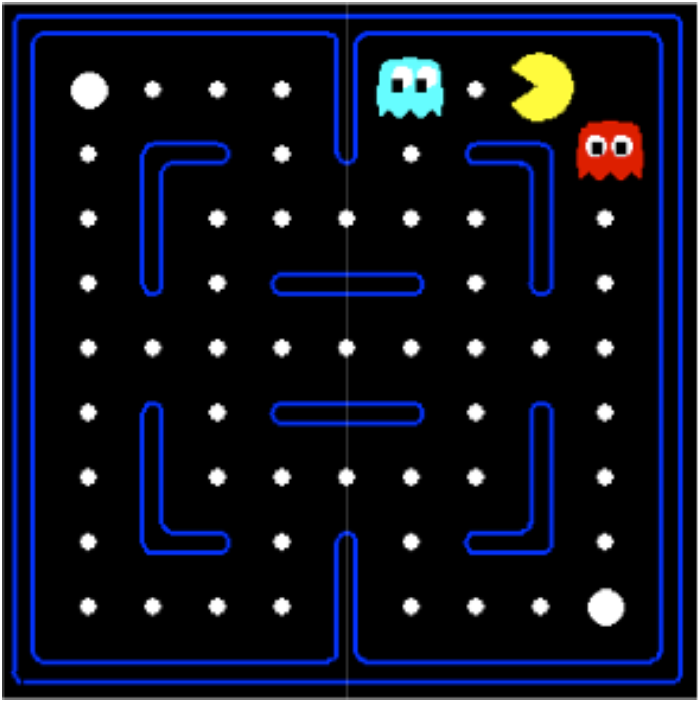
\includegraphics[width=0.35\textwidth]{figures/q72.png}
\end{figure}
\begin{align*}
    f_1(s^{\prime}, west) &= \frac{1}{1} = 1 \\
    f_2(s^{\prime}, west) &= 1 \\
    f_1(s^{\prime}, east) &= \frac{1}{2} = 0.5 \\
    f_2(s^{\prime}, east) &= 1 \\
\end{align*}
Therefore:
\begin{align*}
    Q(s, west) &= 1 \times 2 + 1 \times 8 = 10 \\
    Q(s, east) &= 0.5 \times 2 + 1 \times 8 = 9 \\
\end{align*}
As a result:
\begin{align*}
    sample &= [r + \gamma \max\limits_{a^{\prime}}{Q(s^{\prime}, a^{\prime})}] \\
    &= [9 + 0.8 (10)] \\
    &= 17
\end{align*}

and:

\begin{align*}
    difference &= sample - Q(s, west) \\
    &= 17 - 26 \\
    &= -9
\end{align*}

\subsection{Now provide the update to the weights.}
Let $\alpha = 0.75$.
\begin{align*}
    w_1 &= w_1 + \alpha \times difference \times f_1(s, west)\\
    &= 2 + 0.75 \times (-9) \times 1\\
    &= -4.75\\
    w_2 &= w_2 + \alpha \times difference \times f_2(s, west)\\
    &= 8 + 0.75 \times (-9) \times 3\\
    &= -12.25\\
\end{align*}


\clearpage
\exercise[8]
Pacman is trying to predict the position of a ghost, which has the following transition graph:

\begin{figure}[h!]
    \centering
    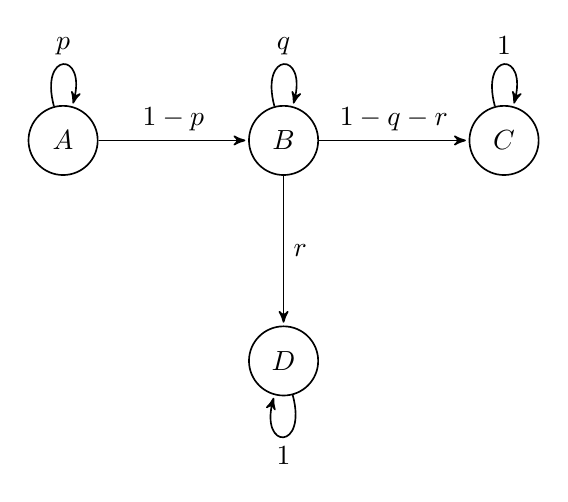
\begin{tikzpicture}[->,>=stealth',shorten >=1pt,auto,node distance=2.8cm, semithick]
  \tikzstyle{every state}=[fill=white,draw=black,text=black]

  \node[state]  (A)              {$A$};
  \node[state]  (B) [right of=A] {$B$};
  \node[state]  (D) [below of=B] {$D$};
  \node[state]  (C) [right of=B] {$C$};

  \path (A) edge [loop above] node {$p$} (A)
            edge              node {$1 - p$} (B)
        (B) edge [loop above] node {$q$} (B)
            edge              node {$1 - q - r$} (C)
            edge              node {$r$} (D)
        (D) edge [loop below] node {1} (D)
        (C) edge [loop above] node {1} (C);
\end{tikzpicture}
\end{figure}

Here, $0 < p < 1$, $0 < q < 1$, and $0 < r < 1$ are arbitrary probabilities. It is known that the ghost always starts in state $A$. For this problem, we consider time to begin at $0$. For example, at time $0$, the ghost is in $A$ with probability $1$, and at time $1$, the ghost is in $A$ with probability $p$ or in $B$ with probability $1 - p$.

\begin{enumerate}
    \item What is the probability that the ghost is in $A$ at time $n$?\\
            \textbf{Answer:} Because once the ghost leaves $A$ there is no way back:\\
            % $P(A, n) = $
            $p^n$
    \item What is the probability that the ghost first reaches $B$ at time $n$?\\
            \textbf{Answer:} Because there is no way back to $B$ from its successors $C$ and $D$, the ghost reaching $B$ at $n$ can only mean the ghost was at $A$ at $n - 1$, therefore:\\ 
            % \\
            % $P_f(B, n) = $
            $(p^{n-1})(1 - p)$ when $n \geq 1$ otherwise $0$. 
            % \\
            % \\
            % Or simply:\\
            % $P_f(B, n) = (1 - p) P(A, n-1)$.
    \item What is the probability that the ghost is in $B$ at time $n$?\\
            \textbf{Answer:} For similar reasons, the ghost being in $B$ at $n$ means it either got to $B$ for the first time, or it reached $B$ at some step less than $n$ and stayed for the remainder:\\
            % $P(B, n) = $
            $\sum\limits_{i=0}^{n - 1}{(p^{i})(1 - p)q^{n - i - 1}}$ when $n \geq 1$ otherwise $0$. 
            % $(p^{n-1})(1 - p) + \sum\limits_{i=1}^{n - 1}{(p^{i-1})(1 - p)q^{n - i - 1}}$ when $n \geq 1$ otherwise $0$. 
            % Or simply:\\
            % $P(B, n) = \sum_{i=1}^{n}{(q ^ {n-i})P_f(B, i)}$.
    \item What is the probability that the ghost first reaches $C$ at time $n$?\\
            \textbf{Answer:} It was in $B$ at $n-1$, and reached $C$ with a probability of $1 - q - r$, therefore:
            % $P_f(C, n) = $
            $[\sum\limits_{i=0}^{n - 2}{(p^{i})(1 - p)q^{n - i - 2}}](1 - q - r) $ when $n \geq 2$ otherwise $0$. 
            % $[((p^{n-1})(1 - p) + \sum\limits_{i=1}^{n - 1}{(p^{i-1})(1 - p)q^{n - i - 1}})](1 - q - r) $ when $n \geq 2$ otherwise $0$. 
            % Or simply:\\
            % $P_f(C, n) = (1 - q - r)P(B, n)$.
    \item What is the probability that the ghost is in $C$ at time $n$?\\
            \textbf{Answer:} For similar reasons, the ghost being in $C$ at $n$ means it either got to $C$ for the first time, or it reached $C$ at some step less than $n$ and stayed for the remainder with probability 1:\\
            $\sum\limits_{j=2}^{n}\big( [\sum\limits_{i=0}^{j - 2}{(p^{\ i \ })(1 - p)q^{\ j - i - 2}}](1 - q - r) \big) $ when $n \geq 2$ otherwise $0$. 
            % $P(C, n) = \sum_{i=2}^{n}{P_f(C, i)}$
\end{enumerate}

\end{document}
 